\documentclass[aps,pre,12pt,preprint,%
	onecolumn,showpacs,showkeys,nofootinbib]{revtex4-1}
%Chinese
	\usepackage[UTF8,fontset=fandol]{ctex}
	\xeCJKsetup{underdot = {
		boxdepth=0pt, format=\huge, depth=.4em
	}}
%	\usepackage[datesep=/]{datetime2} % Use default
	\DeclareTextFontCommand{\textbf}{\sffamily}
%Presenting
	\usepackage[table]{xcolor}
	\usepackage{graphicx}
	\usepackage[space]{grffile}
	\usepackage[font=small,format=plain,%
		labelfont=bf,textfont=it,%
		singlelinecheck=false]{caption}
	\usepackage[above]{placeins}
%	\usepackage{float} % Cause trouble for table footnotes
	\usepackage{wrapfig}
	\usepackage{tabularx,array,booktabs,multirow,bigstrut}
	\newcolumntype{C}[1]{>{\hsize=#1\hsize%
		\centering\arraybackslash}X}
	\newcommand{\minitab}[2][l]{%
		\begin{tabular}{#1}#2\end{tabular}}
	\usepackage{setspace,dcolumn}
	\usepackage{subfig}
	\usepackage{psfrag,epsfig}
%MathSetting
	\let\latexointop\ointop
	\usepackage{amsmath,bm,amssymb,esint,extarrows}
	\usepackage{upgreek,textcomp,mathrsfs}
	\usepackage[only,sslash]{stmaryrd}
	\usepackage{nicefrac,eqnarray}
%	\usepackage{amsthm} % Enable when necessary
%	\usepackage[mathscr]{eucal} % Enable when necessary
	\usepackage{mathtools,physics,siunitx}
	\usepackage{stackengine,varwidth}
	\usepackage{tikz}
	\usepackage{resizegather,empheq}
	\usetagform{default}
	\usepackage{calligra,fourier-orns}
	% Keep \oint unchanged by esint
	\let\ointop\undefined
	\let\ointop\latexointop
	% Define a scriptr 
	\DeclareMathAlphabet{\mathcalligra}{T1}{calligra}{m}{n}
	\DeclareFontShape{T1}{calligra}{m}{n}{<->s*[2.2]callig15}{}
	\newcommand{\scriptr}{\mathcalligra{r}\,}
	\newcommand{\rvector}{\pmb{\mathcalligra{r}}\,}
	% Useful shorthand
	\DeclarePairedDelimiter\ave{\langle}{\rangle}
	\newcommand\inlineeqno{\stepcounter{equation}\ (\theequation)}
	\newcommand{\sinc}{\operatorname{sinc}}
	\newcommand{\mbb}[1]{\mathbb{#1}}
	\newcommand{\mrm}[1]{\mathrm{#1}}
	\newcommand{\mcal}[1]{\mathcal{#1}}
	\newcommand{\tup}[1]{\textup{#1}}
	% Scaling and positioning
	\newcommand\scalemath[2]{\scalebox{#1}{\mbox{\ensuremath{\displaystyle #2}}}}
	\newcommand\raisemath[2]{\raisebox{#1\depth}{${#2}$}}
	\empheqset{box=\nicebox}
	% Presenting
	\newcommand*\nicebox[1]{\fbox{\hspace{1em}\addstackgap[5pt]{#1}\hspace{1em}}}
	\sisetup{%
		redefine-symbols=false,%
		separate-uncertainty=true,%
		range-phrase=\,\textasciitilde\,,%
		arc-separator = \,}
	\allowdisplaybreaks[2]
%ParagraphSetting
	\setlength{\parskip}{.3\baselineskip}
	\usepackage[defaultlines=2,all]{nowidow}
	\postdisplaypenalty=50
%PageSetting
	\usepackage{titlesec}
	\titleformat*{\section}{\large\bfseries}
	\usepackage[colorlinks=true,linkcolor=blue]{hyperref}
	\newcommand{\texstringonly}[1]{%
		\texorpdfstring{#1}{}}
	\usepackage[vmargin={3.5cm,4cm},hmargin=3cm,%
		footnotesep=\baselineskip]{geometry}
%	\usepackage[bottom]{footmisc} % Cause trouble for table footnotes
	\usepackage{changepage}
	% Autoref names
	\renewcommand{\tableautorefname}{\tablename}
	\renewcommand{\figureautorefname}{\figurename}
	% List settings
	\usepackage{enumitem}
	\setlist{itemsep=0pt,topsep=0pt,labelindent=\parindent,leftmargin=0pt,itemindent=*}
	% Some redefined lengths
	\setlength{\headsep}{1.6\baselineskip}
%	\setlength{\footnotesep}{3\parskip} % Use when necessary
	% Header
	\usepackage{fancyhdr,lastpage}
	\pagestyle{fancy}
%	\fancyhf{} % Clear default settings; disabled for now
	\cfoot{--\ \thepage\,/\,\pageref{LastPage} \ --}
	\setlength{\footskip}{2\baselineskip}
	\renewcommand{\headrulewidth}{0.1pt}
	\renewcommand{\headrule}{
		\ifnum\value{page}=1\relax\else
			\vbox to 2pt{
			\hbox to \headwidth{\dotfill}\vss}
		\fi}
	\fancypagestyle{titlepagestyle}{%
		\fancyhead{}
		\chead{
			\vspace{2.5\baselineskip}
			
\includegraphics[width=.75\linewidth]{../PKUPhy}}
	}
	% Separator
	\newcommand{\newparagraph}{\pagebreak[3]\noindent%
		\hfil
		~\raisebox{-4pt}[10pt][10pt]{\decofourright~~~~~~~~\decofourleft}~ %
		\par
	}
%	% Background % Use when necessary
%	\usepackage{background} %Waterstamp package
%	\SetBgContents{...的实验报告} %Waterstamp to prevent copying
%	\SetBgScale{5} %Waterstamp setting
	% Essay format
	\renewcommand\appendixname{附录}
	\renewcommand\abstractname{}%摘要
	\renewcommand\tablename{表}
	\renewcommand\figurename{图}
	\renewcommand\refname{参考文献}
	\makeatletter
	\def\@pacs@name{\songti\zihao{-4}{\bf PACS码:}}
	\def\@keys@name{\songti\zihao{-4}{\bf 关键词:}}
	\def\Dated@name{日期:}
	\def\Received@name{\zihao{-5}{接收} }
	\def\Revised@name{\zihao{-5}{修订} }
	\def\Accepted@name{\zihao{-5}{采纳} }
	\def\Published@name{\zihao{-5}{发表} }
	\makeatother
	\linespread{1.5}
	\renewcommand{\labelenumi}{\alph{enumi}.}
	\leftmargini=20mm
	\newcommand{\supercite}[1]{\textsuperscript{\,%
		[\citenum{#1}]}}
	\let\fancycite\cite
	\renewcommand{\cite}[1]{\textup{\fancycite{#1}}}
	% Math line spacing
	\newlength{\djot}
	\setlength{\djot}{\jot}
	\newcommand{\restorejot}{\setlength{\jot}{\djot}}

%Miscellaneous
%	\newcommand{\tabindent}{\hspace{2em}}
%FourierTransform
	\newcommand{\fourierf}{\mathscr F}
%Atoms
	\newcommand{\SrAtom}{\,\textsuperscript{90}\tup{Sr}\,}
	\newcommand{\Yatom}{\,\textsuperscript{90}\tup{Y}\,}
	\newcommand{\CsAtom}{\,\textsuperscript{137}\tup{Cs}\,}
	\newcommand{\CoAtom}{\,\textsuperscript{60}\tup{Co}\,}
\begin{document}
%Basic Data
	\title{%
	\texstringonly{\hfil\\[2\baselineskip]}
	\sf\LARGE%
		康普顿效应验证实验%
	\texstringonly{\vspace{3ex}}}
	\author{\fangsong\large%
		Bryan%
	\vspace{2mm}}
	\affiliation{\it%
		北京大学物理学院~~学号:\normalfont 1500000000\,}
	\date{\today}
	\keywords{康普顿散射\ 能谱\ 散射截面}
	\email{guesswhat@email.addr;}

\begin{abstract}
\vspace{10mm}
\begin{spacing}{1.5}\normalsize
\setlength{\parskip}{.3\baselineskip}
%	200—300字,
%	说明用什么方法做了什么事,
%	由此得到什么结果和结论,
%	有何意义.
%	不用缩略词,不用第一人称.
%%%%%%%%%%%%%%%%%%%%%%%%%%%%%%%%
	康普顿效应源于电子对高能光子的非弹性散射。光的经典波动理论难以解释这一现象,它强烈地依赖于\textit{波粒二象性}。
	
	本实验以\CsAtom 为放射源,测定了$\SI{662}{\keV}$ $\gamma$射线被铝棒散射后的能量及相对微分散射截面,考察了其关于散射角的分布。
	实验结果表明,散射光子能量及相对微分散射截面均随散射角增大而递减,其规律与理论分析基本一致,从而验证了康普顿效应,进而证实了光的波粒二象性。
\end{spacing}
\end{abstract}

\maketitle
\thispagestyle{titlepagestyle}

%	\item 课程实验报告应假定读者既不是已知全部实验细节的指导教师,也不是缺少专业知识的公众,而是同领域的实验研究者,或审稿人. 不能要求读者要在读过课程讲义后才能读懂课程实验报告.
%	\item 公式、图和表要分别用阿拉伯数字编列序号. 公式和图表要达到可发表的质量.
%	\item 凡不是自己独立思考得到的内容都应该引参考文献. 不能大段引用同一参考文献. 对复杂问题,应该优先考虑引用参考文献得到结果. 对简单一些的问题才鼓励独立思考.
%	\item 较长的推导和说明可以作为附件提交,不占用报告篇幅.
%	\item 思考题不是报告的组成部分. 应另起一页附在报告的最后.
\section{引言}
%%	研究论文引言一般包含以下内容:
%%	(1)所研究领域背景和现状;
%%	(2)有待研究的问题;
%%	(3)本研究的目的、主要内容和结果;
%%	(4)结果的意义.\par
%%	在写实验报告的引言时,同学可以假想自己是第一个做类似研究的人.\par
%%	引言一定要切合报告正文,不能漫无目的地介绍背景. 要快速地将读者引导到报告主题上,并作较深入的讨论.\par
%%	引言篇幅可以在较大范围内变化,但最长不应超过报告文字篇幅的1/3.\par
%%	引言撰写可以参考实验讲义,可以复述,但不能复制讲义上的任何一句话.\par
%%%%%%%%%%%%%%%%%%%%%%%%%%%%%%%
	20世纪早期,诸多实验迹象表明,被物质散射后的X射线能量减小\footnote{%
		详见 \cite{taylor2004modern} 及 \cite{textbook}. 
	};而经典电动力学的预测表明,散射波的能量应当与入射波一致。
	
	1923年,康普顿(A. H. Compton)采用光量子假定,结合狭义相对论的动力学,成功地解释了散射能量的变化\supercite{compton1923quantum}。据此理论可知,光子的能量损失源于与电子的非弹性散射;其有效性在吴有训等人的一系列后续实验(如 \cite{woo1926distribution})被进一步加以证实。
	
	康普顿散射进一步确认了光子正是传递电磁场相互作用的粒子(force carrier)。1928年,Oskar Klein和Yoshita Nishina根据狄拉克(Paul Dirac)的量子电动力学(QED)推导出了散射的微分截面。
	Klein--Nishina公式是QED的最早成果之一,其在低能极限下表征经典的弹性散射(\textit{汤姆逊散射}),而在高能情形下对应康普顿散射。
	
	如今,康普顿散射仍作为研究基本粒子结构的一个重要方法。本实验意在复现康普顿效应的验证过程,通过测定$\gamma$射线的能谱,分析能量及相对微分散射截面随散射角$\theta$的变化,以验证上述理论结果。这也是对吴先生的工作的一次重现。
\section{理论}
	参见\cite{compton1923quantum}, 考虑高能极限,即光子能量远大于电子束缚能,此时电子近似是自由的;由相对论性能动量守恒,光子能量$e = h\nu$, 可得:
	\begin{equation}
		h\nu' = \frac{h\nu}
			{1 + \frac{h\nu}{mc^2}
				\pqty{1 - \cos\theta}}
	\end{equation}
	这里,$m \sim \SI{.511}{\MeV/c^2}$是电子的静质量,$\nu,\nu'$是散射前后光子的频率变化,$h$为普朗克常数,$c$为光速。%
\clearpage
	
	Klein--Nishina公式给出关于立体角元$\Omega$的微分散射截面:
	\begin{equation}
	\begin{aligned}
		\dv{\sigma}{\Omega}
		= r_0^2
		&\left(\frac{1}{1+\alpha\,(1-\cos \theta )}\right)^2
		\left(\frac{1+\cos ^2\theta}{2}\right)\\[1ex]
		&\qquad\times\left(1+\frac{\alpha ^2 (1-\cos\theta )^2}{\pqty\big{1+\cos^2\theta} \pqty\big{1+\alpha\,(1-\cos \theta )}}\right)
	\end{aligned}
	\end{equation}
	这里采用了 \cite{textbook} 给出的形式,其中$r_0 \sim \SI{2.818}{fm}$为电子的经典半径,$\alpha = \frac{h\nu}{mc^2}$. 
	
	考虑实测过程,微分散射截面可表示为:
	\begin{equation}
		\dv{\sigma}{\Omega}
		\propto \frac{N(\theta)}{R(e)\,\eta(e)},\quad
		e = e(\theta)
	\end{equation}
	$N(\theta)$为实测光电峰值计数;由于存在显著的本底,这里\cjkdot{约定}峰的区间为峰值附近、计数$>\frac{1}{3}$峰值的区域。
	
	此外,峰总比$R(e)$及探测效率$\eta(e)$是探测器的属性,它们是能量$e$的函数,从而间接依赖于$\theta$. 比例系数不依赖于散射角$\theta$; 这里我们关注微分散射截面随$\theta$的变化规律,即考察:
	\[ \pqty{\dv{\sigma}{\Omega}}_{\!\!\theta}\,
	\bigg/ \pqty{\dv{\sigma}{\Omega}}_{\!\!\theta_0} \]
\section{实验装置}
%%	在此部分需要将实验条件交待清楚到别人能重复你的实验结果的程度. 此外,还需表明你已尽了最大努力来提高实验精度和结果的可靠性. 简单的不确定度估计可以在此节给出,复杂一些的可以放到分析讨论部分.\par
%%	实验条件不仅是指直接影响实验结果的实验参量,而且还包括影响实验质量和可靠性的因素,如室温、空气湿度、基真空、原材料纯度等.\par
%%	作为教学实验报告,此节写详细一点没有坏处.\par
%%	成段有叙述,必要才分节。
%%%%%%%%%%%%%%%%%%%%%%%%%%%%%%%
	本实验使用\CsAtom 作为放射源,考虑能量 \SI{661}{\keV} 的出射光子,其经准直后打在散射样品——铝棒上,以 NaI (Tl) 探头测得不同角度的能谱信号,进一步分析得到散射光子能量与微分散射截面。
	
	仪器系统由北京核仪器厂生产封装为BH1307型康普顿散射仪,其中NaI (Tl) 探头能够以散射棒为中心而转动,这样不断改变散射角可以测得不同角度下的散射光子能谱。仪器示意图如 \ref{fig:scheme} 所示。
	
	\begin{figure}[!h]
	\centering
	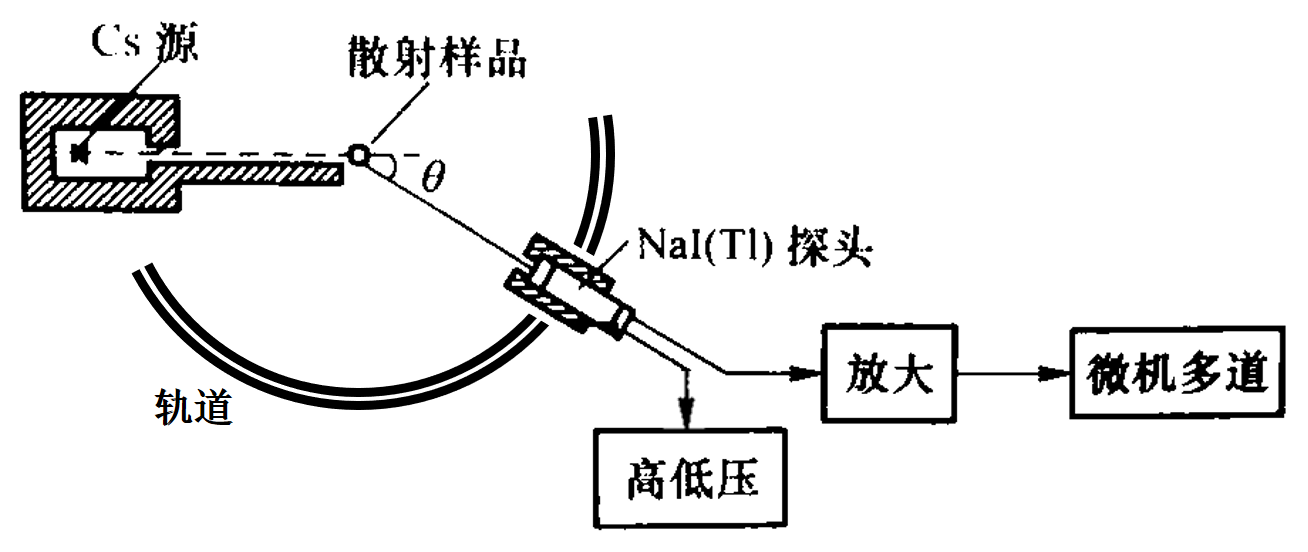
\includegraphics[width=.75\linewidth]{comptonScheme.png}
	\caption[仪器示意图]{康普顿散射仪示意图,%
		参见 \cite{textbook}. }\vspace{1ex}
	\raggedright\small
	\textit{\hphantom{说明}%
		如图所示,实验用\CsAtom 源置于铅盒内,可通过一手柄开关、控制出射通量大小;本实验中的散射样品为铝棒,可从基座上取下;“高低压”指探头的高压调节电路,本实验设定高压 \SI{675}{\V}, 增益\tup{(1.2)}. 实验中,观察到高压示数存在$\pm\SI{1}{\V}$左右的起伏,实际高压示数为 \SIrange{674}{675}{\V}. 
	\vspace{1ex}}
	\label{fig:scheme}
	\end{figure}%
\FloatBarrier
	
	首先,固定$\theta = \ang{0}$, 标定探测系统;利用内置\CsAtom 源 \SI{662}{\keV} 峰及外置\CoAtom 源的 \SI{1.17}{\MeV}, \SI{1.33}{\MeV} 峰实现这一过程。定标过程中,为防止辐射流过大导致系统计数卡死,将\CsAtom 源半开。结果给出道址$x$与能量$e$之间的近似线性关系:
	\[
		\frac{e}{\si{\MeV}}
		= 1.69 + 1.39 x
	\]
	相关性系数$R^2 > \num{.9999}$足够好;在此基础上进行后续实验。
\section{结果与分析}
%	实验结果应尽量以图表的形式给出. 每一个图表都应该是完整的,即阅读图表时可以不必依赖正文.\par
%	依自己意愿,实验结果和对结果的分析讨论既可分为两节也可合在一节.\par
%
%	每个图一般包含:图名、轴名、轴、刻度、标尺、数据点、曲线、图例、标注和图注等部分. 应尽量让读者不看正文就能基本理解图的含意.\par
%	逐点测量得到的函数关系要同时用表格和图给出. 需要作比较的多条曲线要画在同一图上.\par
%	为避免读者在图表和正文间反复跳跃阅读,在正文中也要对图表作必要的说明.\par
%
%	对于预料之外的实验结果,必须首先小心证明其可靠性.读者只有在相信你的实验结果时才愿意花时间看你的分析.\par
%	必须用文字归纳整理出正式的实验结果或结论.可信的实验结果是课程报告最重要的内容.作为一个实验物理工作者,分析解释出错并不丢脸,实验结果不被采信则是致命的.\par
%	教学实验的结论往往是预先知道的. 所以,教师更关心的是你的说理过程. 一般说来,单由课内实验的结果不足以能得到明确的结论. 此时,你可以引用他人的研究结果来帮助帮助自己的论证,但必须注明出处. \par
%	确实不能得到明确结论时,可以给出几种可能结论并指出可以再做哪些实验来帮助作进一步的判断.\par
%	总之,分析讨论部分要做到: 论据要valid,论证要reasonable,结论要convincing.\par
%%%%%%%%%%%%%%%%%%%%%%%%%%%%%%
	依次测定
	$\theta
		= \ang{20},\ang{40},\ang{60},
		\ang{80},\ang{100},\ang{120}$
	时的散射能谱和背景能谱;背景能谱在取下铝散射棒后测得。所得能谱与峰值如下所示。将测定峰值与康普顿的理论预计比较,可见两者吻合得不错,这便初步验证了理论的有效性。
	
	进一步,利用前述公式计算相应的微分散射截面,以$\theta = \ang{20}$情形为准,考察相对截面随$\theta$的变化规律,可见同样与Klein--Nishina公式给出的理论预测一致。
	
	\begin{figure}[!h]
	\vspace{-3.5ex}
	\centering
	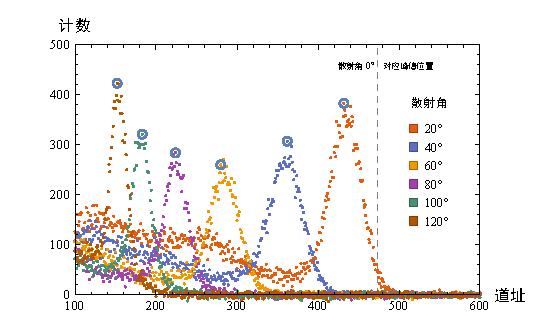
\includegraphics[width=.95\linewidth]{ePlot.pdf}
	\caption[能谱]{\tup{\CsAtom} 源光子被铝棒散射后的能谱,%
		截取峰值附近示意如图。}\vspace{1ex}
	\raggedright\small
	\textit{\hphantom{说明}%
		本能谱已经除去了背景分布,即图中计数值为一定角度下的$\pqty{\textit{散射谱} - \textit{背景谱}}$. \ang{0} 时的能谱是在\tup{\CsAtom} 源半开情况下测得的,其与$\theta > \ang{0}$的能谱之间没有可比性,故在此图中未画出,仅以虚线标记其对应的峰值位置。
	\vspace{-3ex}}
	\label{fig:eDist}
	\end{figure}
	\begin{figure}[!h]
	\centering
	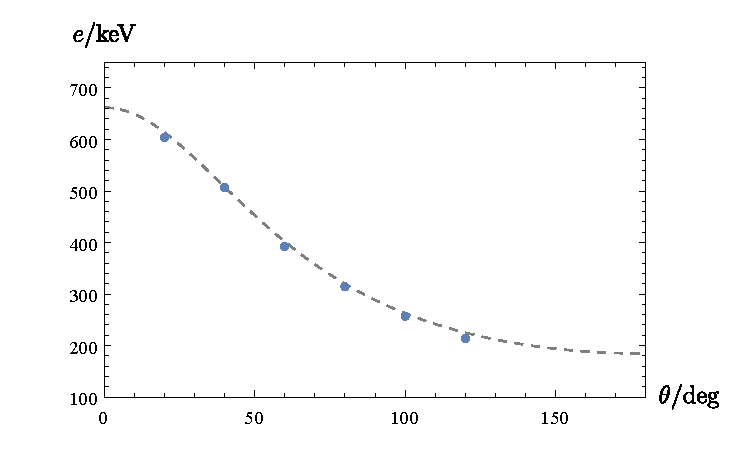
\includegraphics[width=.75\linewidth]{peakCompare.pdf}
	\caption[能峰]{\tup{\CsAtom} 源光子被铝棒散射后的%
		能量峰值角分布}\vspace{1ex}
	\raggedright\small
	\textit{\hphantom{说明}%
		图中以虚线表示理论预测值,以散点表示实测值;可见两者基本吻合。此外,上述实测能量由 \SI{662}{\keV} 值定标给出,因此$\theta = \ang{0}$对应的 \SI{662}{\keV} 不算作实测数据。
	}
	\label{fig:peakGraph}
	\end{figure}%
\FloatBarrier
	
	\begin{figure}[!h]
	\centering
	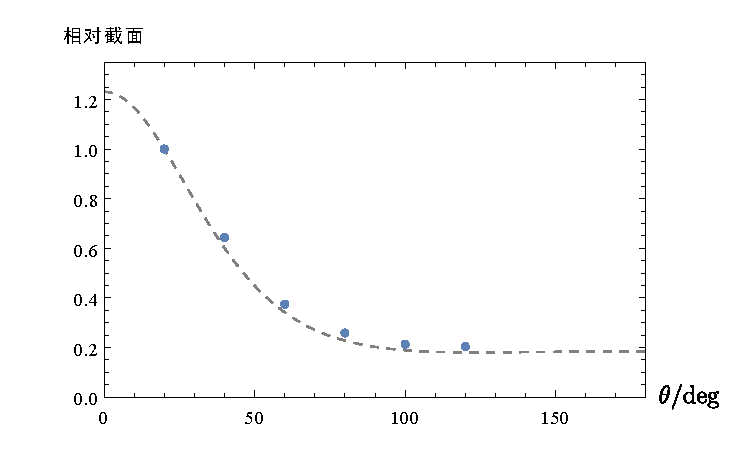
\includegraphics[width=.85\linewidth]{crossSectPlot.pdf}
	\caption[见面]{\tup{\CsAtom} 源光子被铝棒散射后的%
		相对微分散射截面角分布}\vspace{1ex}
	\raggedright\small
	\textit{\hphantom{说明}%
		同样,图中以虚线表示理论预测值,以散点表示实测值;可见两者基本吻合,实测值较理论值有所偏高。此外,相对截面以$\theta = \ang{20}$为标准,即\CJKunderdot{定义}该点的截面等于1, 这一数值也体现在了上图当中。
	\vspace{0ex}}
	\label{fig:crossSection}
	\end{figure}%
\FloatBarrier
	
	具体计算实测数据与理论值的相对偏差,结果如下所示。
	\begin{table}[!h]
	\caption[实测参数]{实测\tup{\CsAtom}源光子%
		被铝棒散射后的能量及相对截面,理论参考值源自 \cite{textbook}. }
	\footnotesize
	\begin{tabularx}{.85\linewidth}{%
		C{.45} | C{1} C{.8} | C{.6} C{.8}}
	 \toprule\midrule
		$\theta/\si{\deg}$ &
		散射光子能量$e/\si{\keV}$ &
		与理论值的偏差 &
		相对截面 &
		与理论值的偏差 \\
	 \midrule
	 20  & 604.1 & $-1.6\%$ & 1     & N/A      \\
	 40  & 506.5 & $-0.3\%$ & 0.643 & $ 7.3\%$ \\
	 60  & 392.1 & $-2.4\%$ & 0.374 & $10.2\%$ \\
	 80  & 314.0 & $-1.8\%$ & 0.258 & $14.0\%$ \\
	 100 & 256.9 & $-2.2\%$ & 0.213 & $13.2\%$ \\
	 120 & 213.6 & $-5.0\%$ & 0.203 & $13.3\%$ \\
	 \midrule\bottomrule
	\end{tabularx}
	\label{tab:coreValues}
	\end{table}%
\FloatBarrier\noindent
	计算过程中,引用了 \cite{textbook} 给出的$R(e),\eta(e)$数据表;表中给出的数据点是离散的,具体的$R(e),\eta(e)$函数由散点数据经三次样条插值给出。
	
	据图线和数据可知,实测能量较理论值普遍\cjkdot{偏低},但偏差不甚显著;而相对截面的偏差则比较显著,且是较实测值\cjkdot{偏高}。简要分析可知,上述偏差应当主要源于实验环境的非理想性;事实上,本实验中有诸多误差来源未能充分控制:
	\begin{enumerate}
	\item 首先,\textbf{能量刻度可能不够精准};本实验中仅取3点标定了系统的能量刻度,相应的线性拟合结果虽具有充分大的相关性系数,但其误差显著,不可忽略;后续可采用更丰富的峰值数据进行定标,以提升能量刻度的准确性。
	\item 此外,\textbf{仪器附近物质中的电子均可参与散射过程},而本实验所在的室内环境不甚空旷,势必对散射能谱造成影响。这一影响并不能通过去除本底而完全消除;事实上,加上铝棒后,散射导致光子的角分布比未加铝棒时显著增大,从而四壁对光子的散射效应增强、角分布更广,导致了额外的散射截面。
	\end{enumerate}
\section{结论}
%%%	首先要给出实验结果,然后再给出由实验结果分析得到的结果和结论.此部分给出的内容要比摘要中的全面,用词要更准确.\par
%%%%%%%%%%%%%%%%%%%%%%%%%%%%%%%
	本实验以\CsAtom 为放射源,考察了 \SI{662}{\keV} 光子散射后的能量角分布及相对微分散射截面角分布,结果与康普顿等人的理论预计基本一致,可以说是验证了康普顿效应。
	
	实验简要分析了可能的误差来源,强调了周围墙体散射可能带来的显著影响;建议更为精确的测定应当在尽可能减小二次散射的空旷环境中进行。
\section{致谢}
%	此部分感谢同组人...和对实验和报告有帮助的人.
%%%%%%%%%%%%%%%%%%%%%%%%%%%%%%
	亲手接触放射源,还是有一些紧张的;感谢楼建玲老师细致而耐心的指导,这给我们带来了巨大的帮助。
\clearpage

\setlength{\bibsep}{2pt}
\linespread{1.2}\selectfont
\bibliographystyle{../BibStyle/gbt-7714-2015-numerical}
\bibliography{../BibStyle/Textbook,bib/Ref}

\clearpage
\end{document}